In this chapter, we will identify and design a controller for the slave motor of the rolling mill. The process is analogous to the master motor, first the motor is identified around the operating point, then a controller is designed which is then simulated and experimentally tested. The reference of the slave motor is the output of the traction controller and the slave motor should thus have good dynamic reference tracking.

\section{Slave Motor}
The right motor is chosen as the slave motor, for the same reason that the left motor was chosen as the master. Figure \ref{fig:RM_RPM_curr} shows the motor's static characteristic and table \ref{tab:RM_operating_region} shows the currents for different operating points.

\begin{figure}[htbp]
\centering
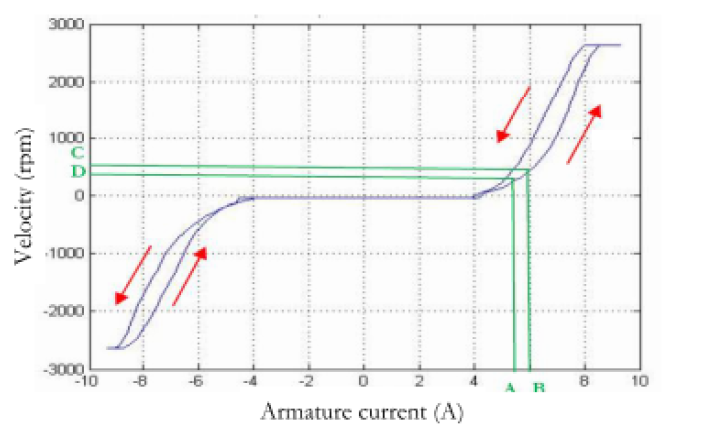
\includegraphics[width = .7\textwidth]{pics/RM_RPM_Current.png}
\caption{Static characteristic of the slave motor}
\label{fig:RM_RPM_curr}
\end{figure}

\begin{table}[H]
	\centering
		\begin{tabular}{lr}
        \toprule
			Armature current [A] & Angular velocity [RPM] \\ \midrule
            5.4 & 244 \\
            5.7 & 370 \\\bottomrule
		\end{tabular}
	\caption{Operating points of the right motor}
	\label{tab:RM_operating_region}
\end{table}

\FloatBarrier

\section{Identification of the Transfer Function}
The slave motor is identified the same way the master motor was. Again, we decide to approximate with a first order system, for the same reasons. Figure \ref{fig:RM_id} shows that transfer function \ref{eq:RM_TF} indeed fits the sample data very well.
\begin{equation}
	RM(s) = \frac{7.128}{6.0665s+1}
    \label{eq:RM_TF}
\end{equation}

\begin{figure}[htbp]
\centering
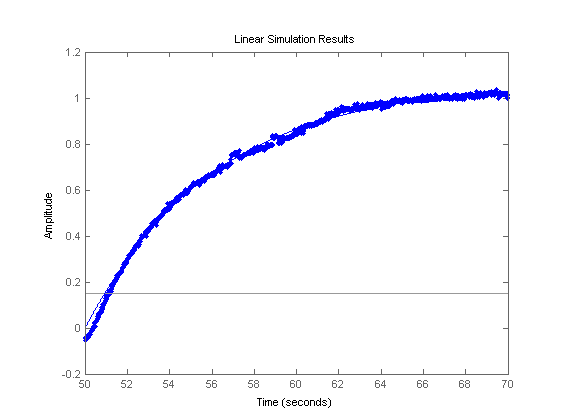
\includegraphics[width = 0.7\textwidth]{pics/RM_systemID.png}
\caption{Sampled and fitted step response of the slave motor}
\label{fig:RM_id}
\end{figure}

\FloatBarrier
\section{Controller Design}
The closed loop needs to be controllable and fast enough to be able to track the tension reference generated by the tension controller. To do this a proportional controller with gain $K$ was chosen. This does not guarantee zero steady state error, but in the case of the slave loop, this is unimportant since it is part of a cascade controller. Furthermore, adding an integrator to the controller slows the response down, which deteriorates tracking.

Figure \ref{fig:RM_rlocus} shows a root locus plot for the right motor. Again, $K$ can theoretically be chosen arbitrarily. It was chosen based on a couple simulations (figures \ref{fig:RM_K2_SIM}, \ref{fig:RM_K3_SIM} and \ref{fig:RM_K4_SIM}) and  practical experiments for different gains (figures \ref{fig:RM_K2},
\ref{fig:RM_K3} and \ref{fig:RM_K4}). None of the simulations have overshoot while some of the practical experiments do (depending on $K$). This is because the transfer function of the motor was reduced to a first order system while in practice it is a non-linear system of higher order.
\begin{figure}[htbp]
\centering
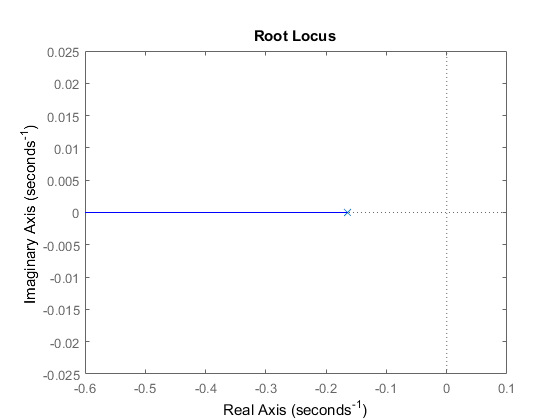
\includegraphics[width = \textwidth]{pics/RM_rlocus.png}
\caption{Root locus plot for the right motor}
\label{fig:RM_rlocus}
\end{figure}

$K = 3$ is chosen since higher gains introduce the risk of putting the actuator in saturation, or at least in a heavily non linear zone.

\begin{figure}[htbp]
\centering
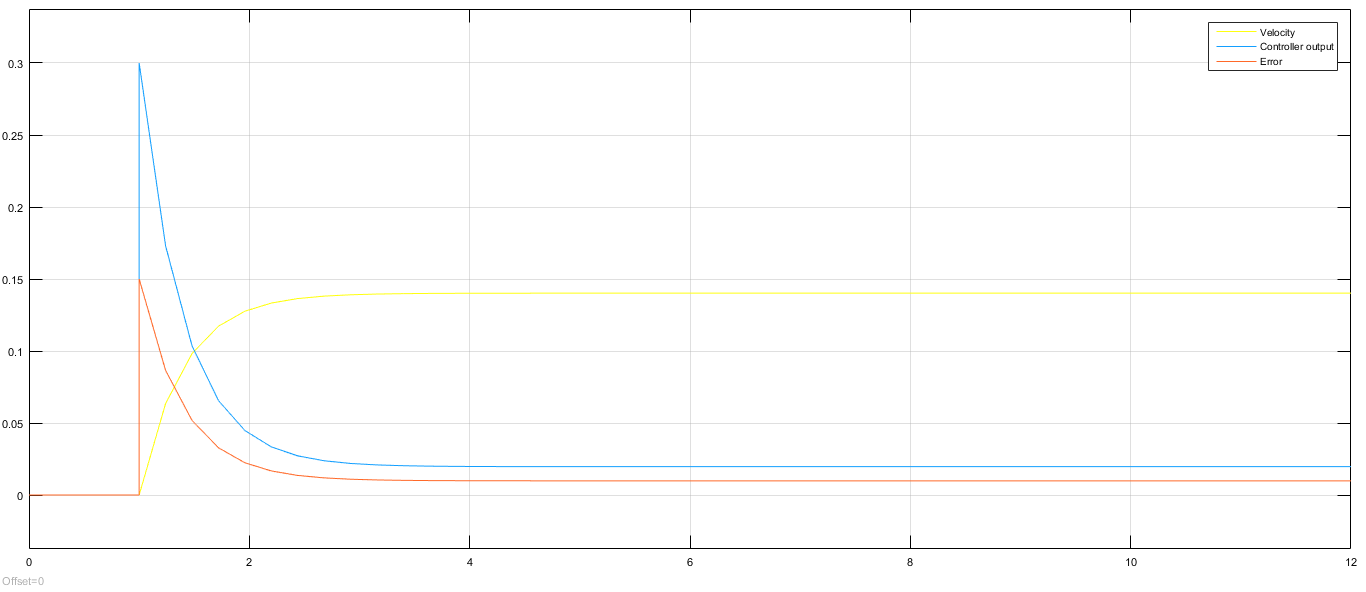
\includegraphics[width = \textwidth]{pics/RM_K2_SIM.png}
\caption{Simulink simulation of the right motor behaviour for $K = 2$}
\label{fig:RM_K2_SIM}
\end{figure}

\begin{figure}[htbp]
\centering
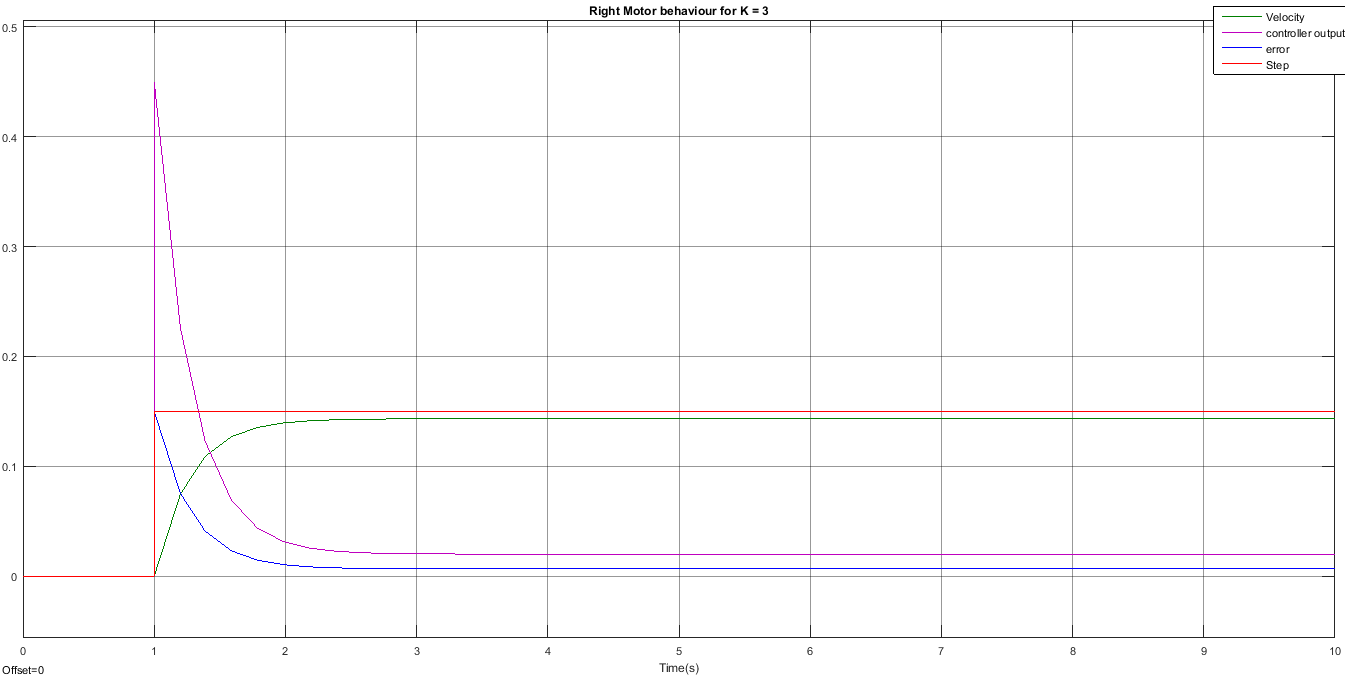
\includegraphics[width = \textwidth]{pics/RM_K3_SIM.png}
\caption{Simulink simulation of the right motor behaviour for $K = 3$}
\label{fig:RM_K3_SIM}
\end{figure}

\begin{figure}[htbp]
\centering
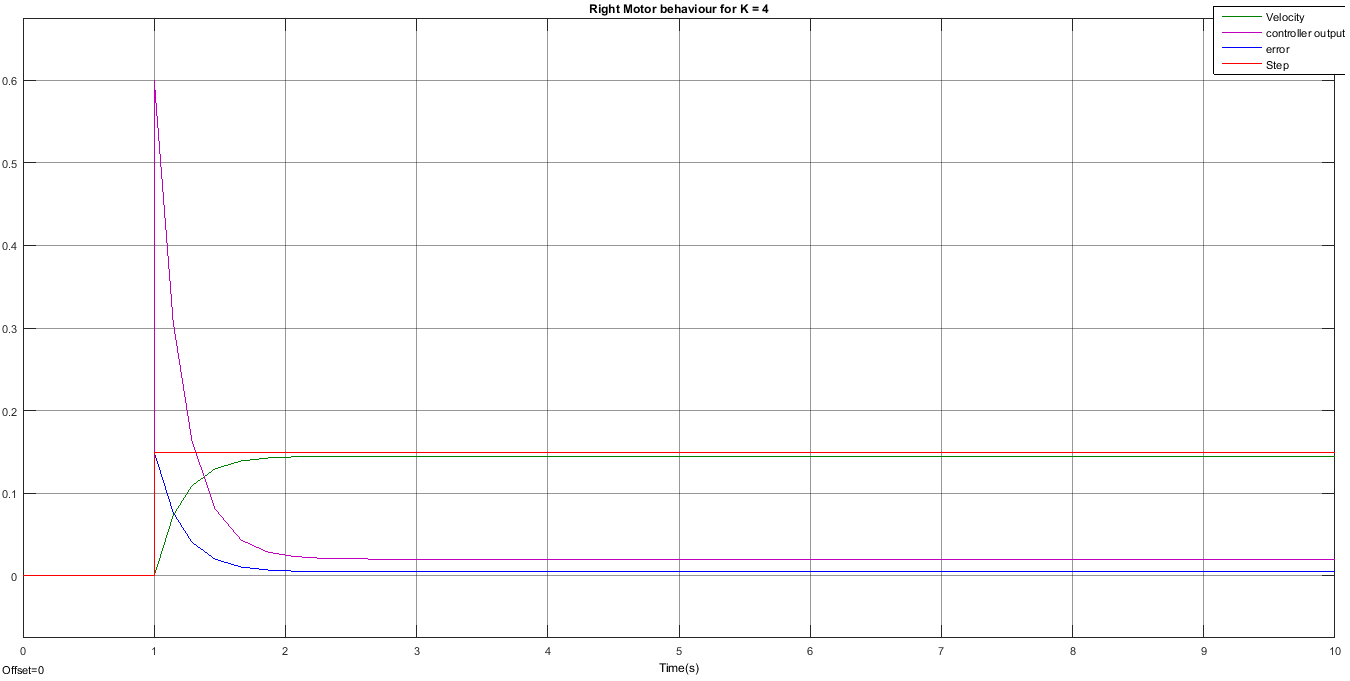
\includegraphics[width = \textwidth]{pics/RM_K4_SIM.png}
\caption{Simulink simulation of the right motor behaviour for $K = 4$}
\label{fig:RM_K4_SIM}
\end{figure}



\begin{figure}[htbp]
\centering
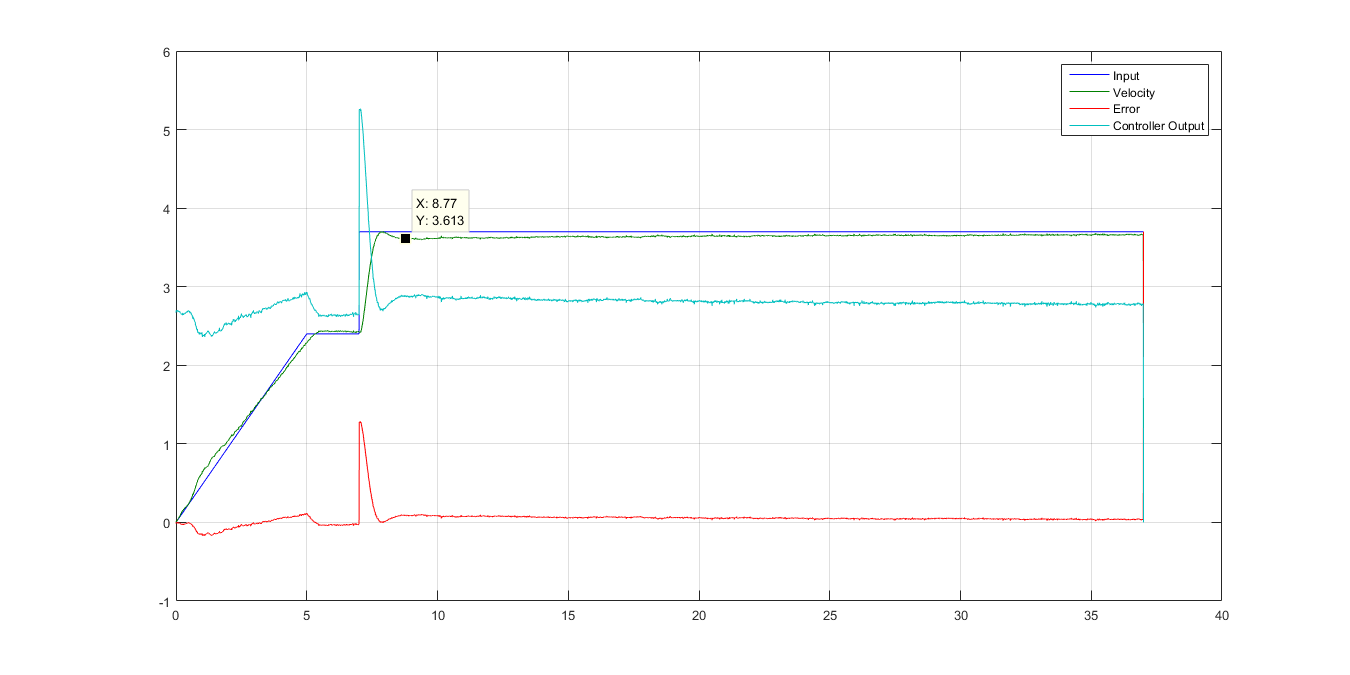
\includegraphics[width = \textwidth]{pics/RM_K2.png}
\caption{Response of the left motor behaviour for $K = 2$ to the blue curve as input.}
\label{fig:RM_K2}
\end{figure}

\begin{figure}[htbp]
\centering
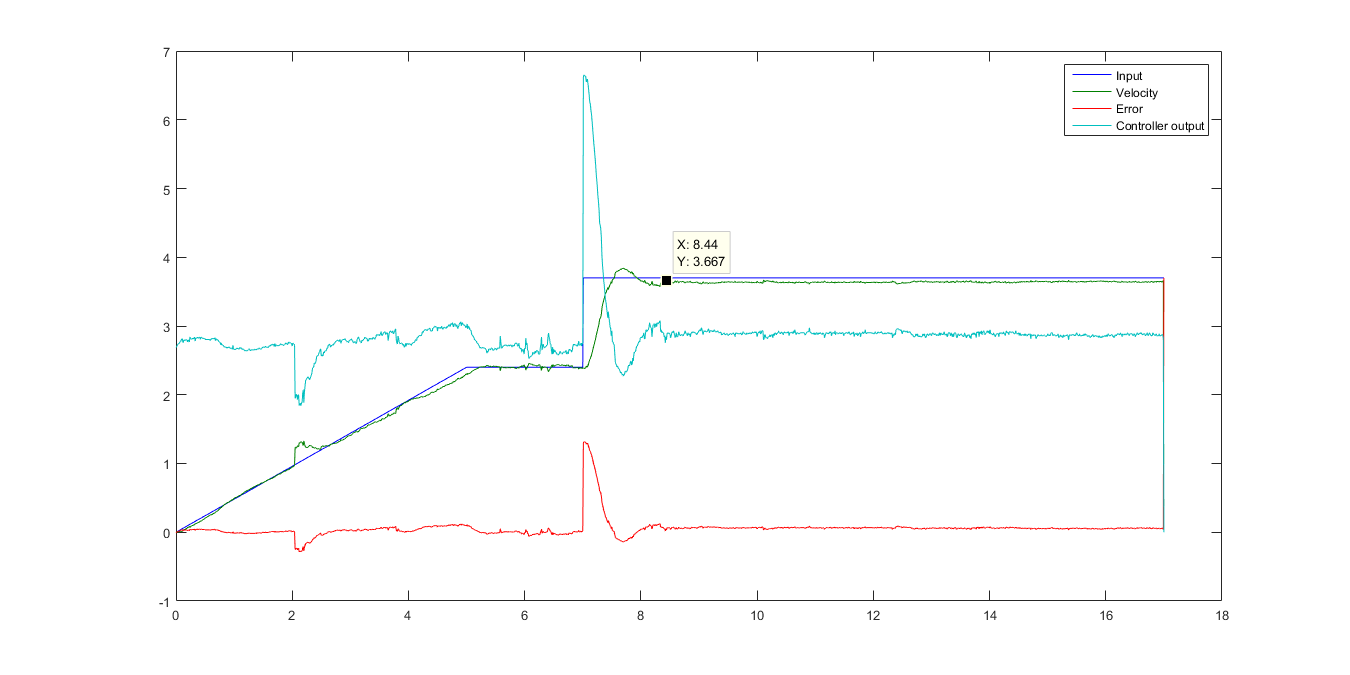
\includegraphics[width = \textwidth]{pics/RM_K3.png}
\caption{Response of the left motor behaviour for $K = 3$ to the blue curve as input.}
\label{fig:RM_K3}
\end{figure}

\begin{figure}[htbp]
\centering
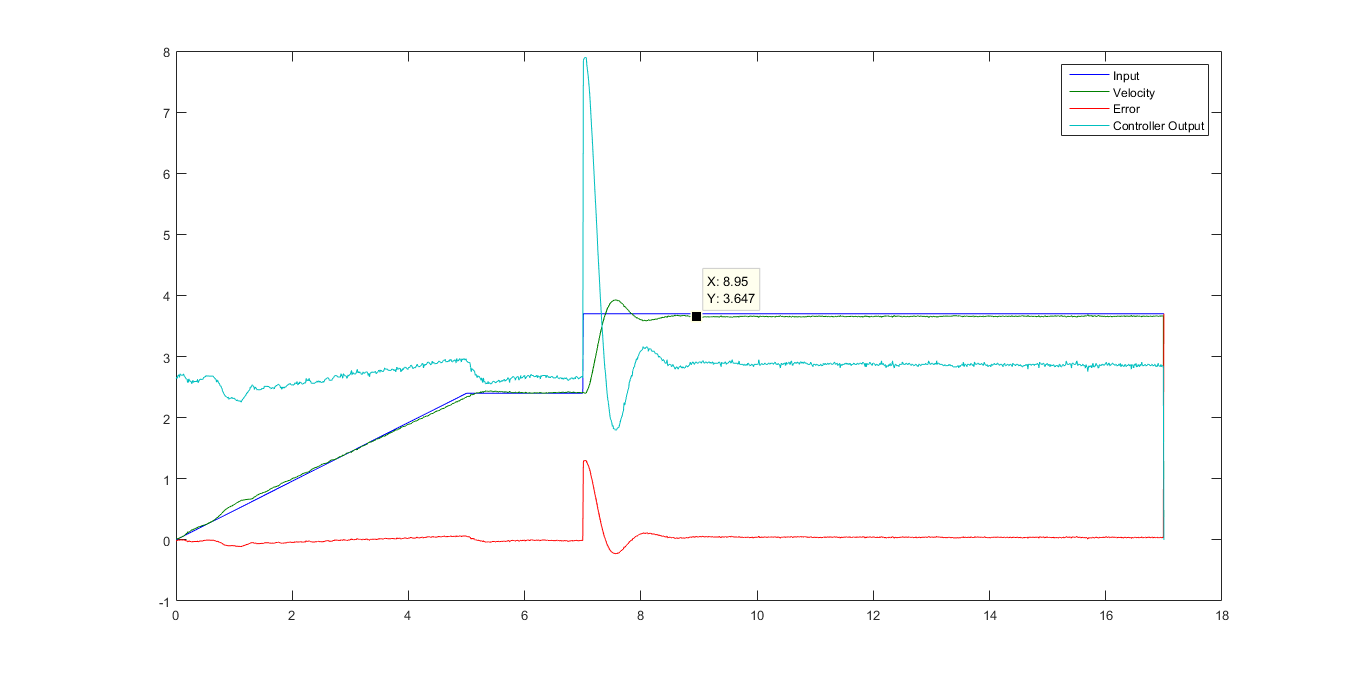
\includegraphics[width = \textwidth]{pics/RM_K4.png}
\caption{Response of the left motor behaviour for $K = 4$ to the blue curve as input.}
\label{fig:RM_K4}
\end{figure}


\section{Conclusions}
A proportional controller was chosen to obtain good reference properties. In a cascade architecture, the steady state error of intern signals is unimportant (but those then need to be monitored along with their reference), so we do not need to introduce an integrator in the controller, which would slow down the response. The outer loop will adjust the slave speed reference in order to obtain zero steady state error on the traction.

As we did for the master motor, the behaviour was identified using a step between two operating points. Using this approximated, transfer function, the controller gain is tuned using simulations and then real-world experiments. Finally a gain of $K = 3$ is selected. We will now design the outer loop controller which will generate the slave speed reference.
